\documentclass[main.tex]{subfiles}
\begin{document}
\paragraph{Nota sulla divisione in componenti di un vettore}
Prendiamo in considerazione quattro esempi:

\begin{enumerate}
	\item Asta orizzontale con forza agente sul lato in alto, inclinata.
	\item Asta orizzontale con forza agente sul lato in basso, inclinata.
	\item Asta inclinata con forza agente sul lato in alto, inclinata.
	\item Asta inclinata con forza agente sul lato in basso, inclinata.
\end{enumerate}

\subparagraph{1) Asta orizzontale con forza agente sul lato in alto, inclinata}
La forza $\vec{F}$ viene applicata nel punto B con un angolo $\alpha<\pi$ (figura \ref{asta_orizzontale_forza_inclinata_alto_intera}).

Dobbiamo ricondurre questa forza nelle sue componenti di \textit{taglio} e \textit{sforzo normale} (figura \ref{asta_orizzontale_forza_inclinata_alto_separata}), per cui, usando della cara vecchia trigonometria si ottiene:
\[
	\vec{F}: \begin{cases}
		N_F = \abs{F}\cos{\alpha}\\
		T_F = \abs{F}\sin{\alpha}
	\end{cases}
\]


\begin{figure}[!tbp]
  \begin{subfigure}[b]{.5\textwidth}
  \centering
  \resizebox{.5\textwidth}{!}{% First image 2015 06 29

\begin{tikzpicture}

  \tiny

  \point{a}{0}{0};
  \point{b}{1}{0};
  \point{c}{2}{0};

  \point{f}{1.866}{0.5};

  \beam{2}{a}{c};

  % \load{1}{a}[240][0.5];
  % \load{1}{a}[150][0.866];

  \load{1}{b}[30][1][0.05]

  \addon{3}{b}{f}{c}[-1];

  % \notation{1}{g}{$\vec{F}$}[above right];
  % \notation{1}{f}{$2\vec{F}$}[above left];
  % \notation{1}{d}{$\vec{F}$}[above right];

  % Degrees
  \notation{1}{b}{$\alpha$}[above right=0.4];
  \notation{1}{b}{$\vec{F}$}[above];

  \notation{1}{a}{A}[below];
  \notation{1}{b}{B}[below];
  \notation{1}{c}{C}[below];

\end{tikzpicture}}
  \caption{Asta orizzontale con forza agente sul lato in alto, inclinata.}
  \label{asta_orizzontale_forza_inclinata_alto_intera}
  \end{subfigure}
  \hfill
  \begin{subfigure}[b]{.5\textwidth}
  \centering
  \resizebox{.5\textwidth}{!}{% First image 2015 06 29

\begin{tikzpicture}

  \tiny

  \point{a}{0}{0};
  \point{b}{1}{0.15};
  \point{c}{2}{0};
  \point{n}{1.6}{0};

  \beam{2}{a}{c};

  \load{1}{b}[0][0.866]
  \load{1}{b}[90][0.5][-0.05]

  \notation{1}{a}{A}[below];
  \notation{1}{b}{B}[below=0.15];
  \notation{1}{c}{C}[below];

  \notation{1}{b}{$\vec{T_F}$}[above left];
  \notation{1}{n}{$\vec{N_F}$}[above=0.11];

\end{tikzpicture}}
  \caption{Asta orizzontale con forza agente sul lato in alto, separata in componenti.}
  \label{asta_orizzontale_forza_inclinata_alto_separata}
  \end{subfigure}
  \caption{Asta orizzontale con forza agente sul lato in alto}
  \label{asta_orizzontale_forza_inclinata_alto}
\end{figure}

\subparagraph{2) Asta orizzontale con forza agente sul lato in basso, inclinata}
La forza $\vec{F}$ viene applicata nel punto B con un angolo $\alpha<0$ (figura \ref{asta_orizzontale_forza_inclinata_basso_intera}).

Dobbiamo nuovamente ricondurre questa forza nelle sue componenti di \textit{taglio} e \textit{sforzo normale} (figura \ref{asta_orizzontale_forza_inclinata_basso_separata}), per cui, usando della cara vecchia trigonometria, ricordando le regole per angoli $>\pi$ si ottiene:
\[
	\vec{F}: \begin{cases}
		N_F = \abs{F}\cos{(2\pi - \alpha)}\\
		T_F = \abs{F}\sin{(2\pi-\alpha)}
	\end{cases}
	\Longrightarrow
	\begin{cases}
		N_F = \abs{F}\cos{\alpha}\\
		T_F = -\abs{F}\sin{\alpha}
	\end{cases}
\]

\begin{figure}[!tbp]
  \begin{subfigure}[b]{.5\textwidth}
  \centering
  \resizebox{.5\textwidth}{!}{% First image 2015 06 29

\begin{tikzpicture}

  \tiny

  \point{a}{0}{0};
  \point{b}{1}{0};
  \point{c}{2}{0};

  \point{f}{1.866}{-0.5};

  \beam{2}{a}{c};

  % \load{1}{a}[240][0.5];
  % \load{1}{a}[150][0.866];

  \load{1}{b}[-30][1][0.05]

  \addon{3}{b}{f}{c}[-1];

  % \notation{1}{g}{$\vec{F}$}[above right];
  % \notation{1}{f}{$2\vec{F}$}[above left];
  % \notation{1}{d}{$\vec{F}$}[above right];

  % Degrees
  \notation{1}{b}{$\alpha$}[below right=0.4];
  \notation{1}{b}{$\vec{F}$}[below];

  \notation{1}{a}{A}[above];
  \notation{1}{b}{B}[above];
  \notation{1}{c}{C}[above];

\end{tikzpicture}}
  \caption{Asta orizzontale con forza agente sul basso in alto, inclinata.}
  \label{asta_orizzontale_forza_inclinata_basso_intera}
  \end{subfigure}
  \hfill
  \begin{subfigure}[b]{.5\textwidth}
  \centering
  \resizebox{.5\textwidth}{!}{% First image 2015 06 29

\begin{tikzpicture}

  \tiny

  \point{a}{0}{0};
  \point{b}{1}{-0.15};
  \point{c}{2}{0};
  \point{n}{1.6}{0};

  \beam{2}{a}{c};

  \load{1}{b}[0][0.866]
  \load{1}{b}[-90][0.5][-0.05]

  \notation{1}{a}{A}[above];
  \notation{1}{b}{B}[above=0.15];
  \notation{1}{c}{C}[above];

  \notation{1}{b}{$\vec{T_F}$}[below left];
  \notation{1}{n}{$\vec{N_F}$}[below=0.11];

\end{tikzpicture}}
  \caption{Asta orizzontale con forza agente sul lato in basso, separata in componenti.}
  \label{asta_orizzontale_forza_inclinata_basso_separata}
  \end{subfigure}
  \caption{Asta orizzontale con forza agente sul lato in basso}
  \label{asta_orizzontale_forza_inclinata_basso}
\end{figure}

\subparagraph{3) Asta inclinata con forza agente sul lato in alto, inclinata.}
La forza $\vec{F}$ viene applicata nel punto B con un angolo $\alpha>0$ (figura \ref{asta_inclinata_forza_inclinata_alto_intera}) su di un'asta inclinata di un angolo $\beta$.

È necessario calcolare l'angolo $\alpha$ con un sistema di riferimento solidale con l'asta AC, per cui ruotato di $\beta$.

\[
	\vec{F}: \begin{cases}
		N_F = \abs{F}\cos{\alpha}\\
		T_F = \abs{F}\sin{\alpha}
	\end{cases}
\]


\begin{figure}[!tbp]
  \begin{subfigure}[b]{.5\textwidth}
  \centering
  \resizebox{.5\textwidth}{!}{% First image 2015 06 29

\begin{tikzpicture}

  \tiny

  \point{a}{0}{0};
  \point{b}{0.5}{0.866};
  \point{c}{1}{2*0.866};

  \point{f}{0.5}{2};

  \point{h}{2}{0}

  \beam{2}{a}{c};

  % \load{1}{a}[240][0.5];
  % \load{1}{a}[150][0.866];

  \load{1}{b}[90][1][0.05]

  \addon{3}{b}{f}{c}[-1];

  \addon{3}{a}{b}{h}[-1];

  % \notation{1}{g}{$\vec{F}$}[above right];
  % \notation{1}{f}{$2\vec{F}$}[above left];
  % \notation{1}{d}{$\vec{F}$}[above right];

  % Degrees
  \notation{1}{b}{$\alpha$}[above left=0.4];
  \notation{1}{a}{$\beta$}[above right=0.4];
  \notation{1}{b}{$\vec{F}$}[above left];

  \notation{1}{a}{A}[below right];
  \notation{1}{b}{B}[below right];
  \notation{1}{c}{C}[below right];

\end{tikzpicture}}
  \caption{Asta inclinata con forza agente sul alto in alto, inclinata.}
  \label{asta_inclinata_forza_inclinata_alto_intera}
  \end{subfigure}
  \hfill
  \begin{subfigure}[b]{.5\textwidth}
  \centering
  \resizebox{.5\textwidth}{!}{% First image 2015 06 29

\begin{tikzpicture}

  \tiny

  \point{a}{0}{0};
  \point{b}{0.5-0.15}{0.866+0.025};
  \point{c}{1}{2*0.866};

  \point{f}{0.5}{2};

  \beam{2}{a}{c};

  % \load{1}{a}[240][0.5];
  % \load{1}{a}[150][0.866];

  \load{1}{b}[60][0.866][0.05]
  \load{1}{b}[150][0.5][0.05]


  % \notation{1}{g}{$\vec{F}$}[above right];
  % \notation{1}{f}{$2\vec{F}$}[above left];
  % \notation{1}{d}{$\vec{F}$}[above right];

  % Degrees
  % \notation{1}{b}{$\alpha$}[above left=0.4];
  % \notation{1}{b}{$\vec{F}$}[above left];

  \notation{1}{a}{A}[below right];
  \notation{1}{b}{B}[below right = 0.15];
  \notation{1}{c}{C}[below right];

\end{tikzpicture}}
  \caption{Asta inclinata con forza agente sul lato in alto, separata in componenti.}
  \label{asta_inclinata_forza_inclinata_alto_separata}
  \end{subfigure}
  \caption{Asta inclinata con forza agente sul lato in alto}
  \label{asta_inclinata_forza_inclinata_alto}
\end{figure}

\subparagraph{4) Asta inclinata con forza agente sul lato in basso, inclinata.}
La forza $\vec{F}$ viene applicata nel punto B con un angolo $\alpha<0$ (figura \ref{asta_inclinata_forza_inclinata_basso_intera}) su di un'asta inclinata di un angolo $\beta$.

È necessario calcolare l'angolo $\alpha$ con un sistema di riferimento solidale con l'asta AC, per cui ruotato di $\beta$.

\[
  \vec{F}: \begin{cases}
    N_F = \abs{F}\cos{(2\pi-\alpha)}\\
    T_F = \abs{F}\sin{(2\pi-\alpha)}
  \end{cases}
  \Longrightarrow
	\begin{cases}
		N_F = \abs{F}\cos{\alpha}\\
		T_F = -\abs{F}\sin{\alpha}
	\end{cases}
\]


\begin{figure}[!tbp]
  \begin{subfigure}[b]{.5\textwidth}
  \centering
  \resizebox{.5\textwidth}{!}{% First image 2015 06 29

\begin{tikzpicture}

  \tiny

  \point{a}{0}{0};
  \point{b}{0.5}{0.866};
  \point{c}{1}{2*0.866};

  \point{f}{0.5}{0};

  \point{h}{2}{0}

  \beam{2}{a}{c};

  % \load{1}{a}[240][0.5];
  % \load{1}{a}[150][0.866];

  \load{1}{b}[-90][1][0.05]

  \addon{3}{b}{f}{c}[-1];

  \addon{3}{a}{b}{h}[-1];

  % \notation{1}{g}{$\vec{F}$}[above right];
  % \notation{1}{f}{$2\vec{F}$}[above left];
  % \notation{1}{d}{$\vec{F}$}[above right];

  % Degrees
  \notation{1}{b}{$\alpha$}[above right=0.4];
  \notation{1}{a}{$\beta$}[below right];
  \notation{1}{b}{$\vec{F}$}[below right=0.3];

  \notation{1}{a}{A}[above left];
  \notation{1}{b}{B}[above left];
  \notation{1}{c}{C}[above left];

\end{tikzpicture}}
  \caption{Asta inclinata con forza agente sul basso in basso, inclinata.}
  \label{asta_inclinata_forza_inclinata_basso_intera}
  \end{subfigure}
  \hfill
  \begin{subfigure}[b]{.5\textwidth}
  \centering
  \resizebox{.5\textwidth}{!}{% First image 2015 06 29

\begin{tikzpicture}

  \tiny

  \point{a}{0}{0};
  \point{b}{0.5+0.15}{0.866+0.025};
  \point{c}{1}{2*0.866};

  \point{f}{0.5}{2};

  \beam{2}{a}{c};

  % \load{1}{a}[240][0.5];
  % \load{1}{a}[150][0.866];

  \load{1}{b}[60][0.866][0.05]
  \load{1}{b}[-30][0.5][0.05]


  % \notation{1}{g}{$\vec{F}$}[above right];
  % \notation{1}{f}{$2\vec{F}$}[above left];
  % \notation{1}{d}{$\vec{F}$}[above right];

  % Degrees
  % \notation{1}{b}{$\alpha$}[above left=0.4];
  % \notation{1}{b}{$\vec{F}$}[above left];

  \notation{1}{a}{A}[above left];
  \notation{1}{b}{B}[above left = 0.15];
  \notation{1}{c}{C}[above left];

\end{tikzpicture}}
  \caption{Asta inclinata con forza agente sul lato in basso, separata in componenti.}
  \label{asta_inclinata_forza_inclinata_basso_separata}
  \end{subfigure}
  \caption{Asta inclinata con forza agente sul lato in basso}
  \label{asta_inclinata_forza_inclinata_basso}
\end{figure}

\end{document}